
% This paper can be formatted using the peerreviewca
% (instead of conference) mode.
\documentclass[conference]{IEEEtran}


\usepackage{graphicx}  % Written by David Carlisle and Sebastian Rahtz


\usepackage{subfigure} % Written by Steven Douglas Cochran

\usepackage{url}       % Written by Donald Arseneau

\usepackage{array}
% There should be no need to do such things with IEEEtran.cls V1.6 and later.
\graphicspath{ {C:/Users/husai/OneDrive/Desktop/Mini Project/} }
% correct bad hyphenation here
\hyphenation{op-tical net-works semi-conduc-tor IEEEtran}


\begin{document}
	
	% paper title
	\title{Implementation of Security System using Computer Vision and Temperature Detection}
	
	
	% author names and affiliations
	% use a multiple column layout for up to three different
	% affiliations
	\author{
		Aryan Dali\\
		\textit{Department of Electronics}\\
		\textit{and Telecommunications}\\
		\textit{Sardar Patel Institute of Technology}\\
		Mumbai, India\\
		aryan.dali@spit.ac.in
		\and
		Jai Damani\\
		\textit{Department of Electronics}\\
		\textit{and Telecommunications}\\
		\textit{Sardar Patel Institute of Technology}\\
		Mumbai, India\\
		jai.damani@spit.ac.in
		\and
		Husain Challawala\\
		\textit{Department of Electronics}\\
		\textit{and Telecommunications}\\
		\textit{Sardar Patel Institute of Technology}\\
		Mumbai, India\\
		husain.challawala@spit.ac.in\\

	}
	
	
	% make the title area
	\maketitle
	
	\begin{abstract}
		\textbf{Providing security and safe access to workplaces has always     been a primary concern for
			corporate and private organizations. Over the years,
			there have been innovations in the way security is
			provided, ranging from keypads to fingerprint sensors.
			However, even these have their lapses and
			shortcomings. A stronger approach to provide
			authorized access is to make use of Computer Vision. This project attempts to implement a Security system which makes use of this software and a
			temperature sensing module to provide a secure,
			monitored and authorized access. The facial recognition
			is achieved with a help of a webcam connected with our system and a python program on which this is executed,
			after which the main control is transferred to the Arduino
			Microcontroller board which tests the two incoming
			inputs and provides access based on its decision. A training model is employed which studies the given
			images of the users and detects them when required.\\}
	\end{abstract}
	
	% no keywords
	\begin{keywords}
		Facial Recognition, Security System, Temperature
		detection, OpenCV, Computer Vision, Arduino, Computer Vision
	\end{keywords}
	
	\IEEEpeerreviewmaketitle
	
	
	
	\section{Introduction}
	% no \PARstart
	In our modern era, physical security risks are at an all-time high. Premises ranging from residential homes to commercial
	buildings require trustworthy and high standard security
	to prevent breach and theft. Hence, we have
	designed a facial recognition security system to grant
	access only to authorized people. This system is considerably more
	efficient than a password-based system or a fingerprint
	system and it also eliminates all the need for any physical contact with the system which is of utmost importance in today's day and age owing to the COVID-19 pandemic.
	The proposed system is a facial recognition security system with a temperature sensor that will be able to protect people’s
	personal spaces as well as their health. It consists of the
	following components: \\
	1. A facial recognition system implemented using python's Computer Vision \\
	2. A temperature sensing system with the help of LM-
	35 temperature sensor. \\
	3. Arduino Microcontroller which oversees the logic.
	
	
	
	\subsection{Motivation}
	As security breaches are becoming a rising concern, a foolproof method is required to curb attacks and improve the standard of overall security that a system provides. Traditional means of security that include the use of a keypad or a fingerprint, though effective, can be compromised easily. Such situations require a stronger means of protection, which uses a person’s face for recognition and authorization. Systems in smartphones and other devices are already incorporating a facial lock system. Additionally, our recent endemic has brought attention to contactless systems and temperature checks at every entrance. This system has improved scalability and can be extended to other areas too. Our motive is to build a secure system which uses facial recognition and contactless to provide access. This system has greater complexity in implementation but offers a better security solution for private as well as public places.
	
	\subsection{Literature Survey}
	The following research papers were studied for the sake of the current project-
	\begin{itemize}
		\item\textbf{Digital Thermometer using Atmega 8
			microcontroller}\cite{a} \\This paper contains information about a
		regular thermometer and its principles,
		LM-35 temperature sensor and the Atmega
		8 microcontroller. It also tells us how to
		connect the microcontroller and the sensor
		to make the digital thermometer
		\item \textbf{Automatic temperature Control System using
			Arduino}\cite{b} \\Using Arduino Uno and LM35
		temperature sensor the author creates a
		control system based on the room
		temperature
		\item \textbf{Face Detection and Recognition using OpenCV
			and Python}\cite{d} \\This research paper provides an ideal way of
		detecting and recognizing facial data
		using OpenCV, and python which is part of
		deep learning. This report will contain a
		proposed system which will help in
		detecting the human face in real time. This
		implementation can be used at various
		platforms in several software applications.
	\end{itemize}
	\subsection{Contributions}
	The primary objectives of the project are as follows-
	\begin{itemize}
		\item To develop a facial recognition security system
		which is trustworthy and efficient.
		\item To make a temperature sensing system to determine
		the temperature and prevent the spread of
		coronavirus.
	\end{itemize}
	\subsection{Outline}
	\begin{itemize}
		\item The paper gives a basic idea about our project, the
		algorithm and the implementation.
		\item The idea is to build a face detection security system
		along with a temperature system.
		\item We also discuss about Python and OpenCV along
		with Arduino.
		\item Lastly, we discuss the results that we obtained.
	\end{itemize}
	
	\section{Body}
	\subsection{Working and algorithm}
	Designing a Facial Recognition based Security System has
	several intermittent stages. Our system basically checks the users face for a match thereby sending a signal to the microprocessor (using the binary system of 1s and 0s) to allow or deny the user permission.
	After this we have used the Arduino microprocessor for
	receiving the signal from OpenCV \cite{e} and executing the
	conditional check and displaying the results of our test cases. Arduino can essentially be described as an open-source platform that is used for simulating electronics projects. It consists of an IDE (Integrated Development Environment) that can run on your computer and is used to write and upload computer code to the physical board \cite{h}. For our purpose, we used an online simulation software called Proteus instead of
	a physical board.
	\\If the signal received is ‘1’ and if the temperature check performed by the LM35 temperature sensor falls under our threshold range, a “Access Granted” prompt would be displayed on the LCD screen attached to our simulation circuit.
	\\Conversely, if there isn't a match in the face and the system sends a ‘0’ to our Arduino circuit, then this implies that it's an unregistered person and thus should not be granted access. And thus, an “Access Denied” prompt is generated on the screen. The LM35 is used to sense and display the temperature \cite{c} of the test case. After giving us the temperature, we constructed a conditional statement in our Arduino code which combines the two criteria for allowing access to a user by using an ‘if’ statement. This implies that even if the face of the person matches that with our database but the temperature lies above a certain value (which is to say that he or she bear the risk of being COVID positive), access would still not be granted to the person by the message “Temperature is too high” being
	displayed on the LCD screen.
	\\In this way we established a double security check on our system by integrating a temperature check and a facial recognition check and combining it on our circuit using the set of applications mentioned above.
	%\centering
	\begin{figure}
		\centering
		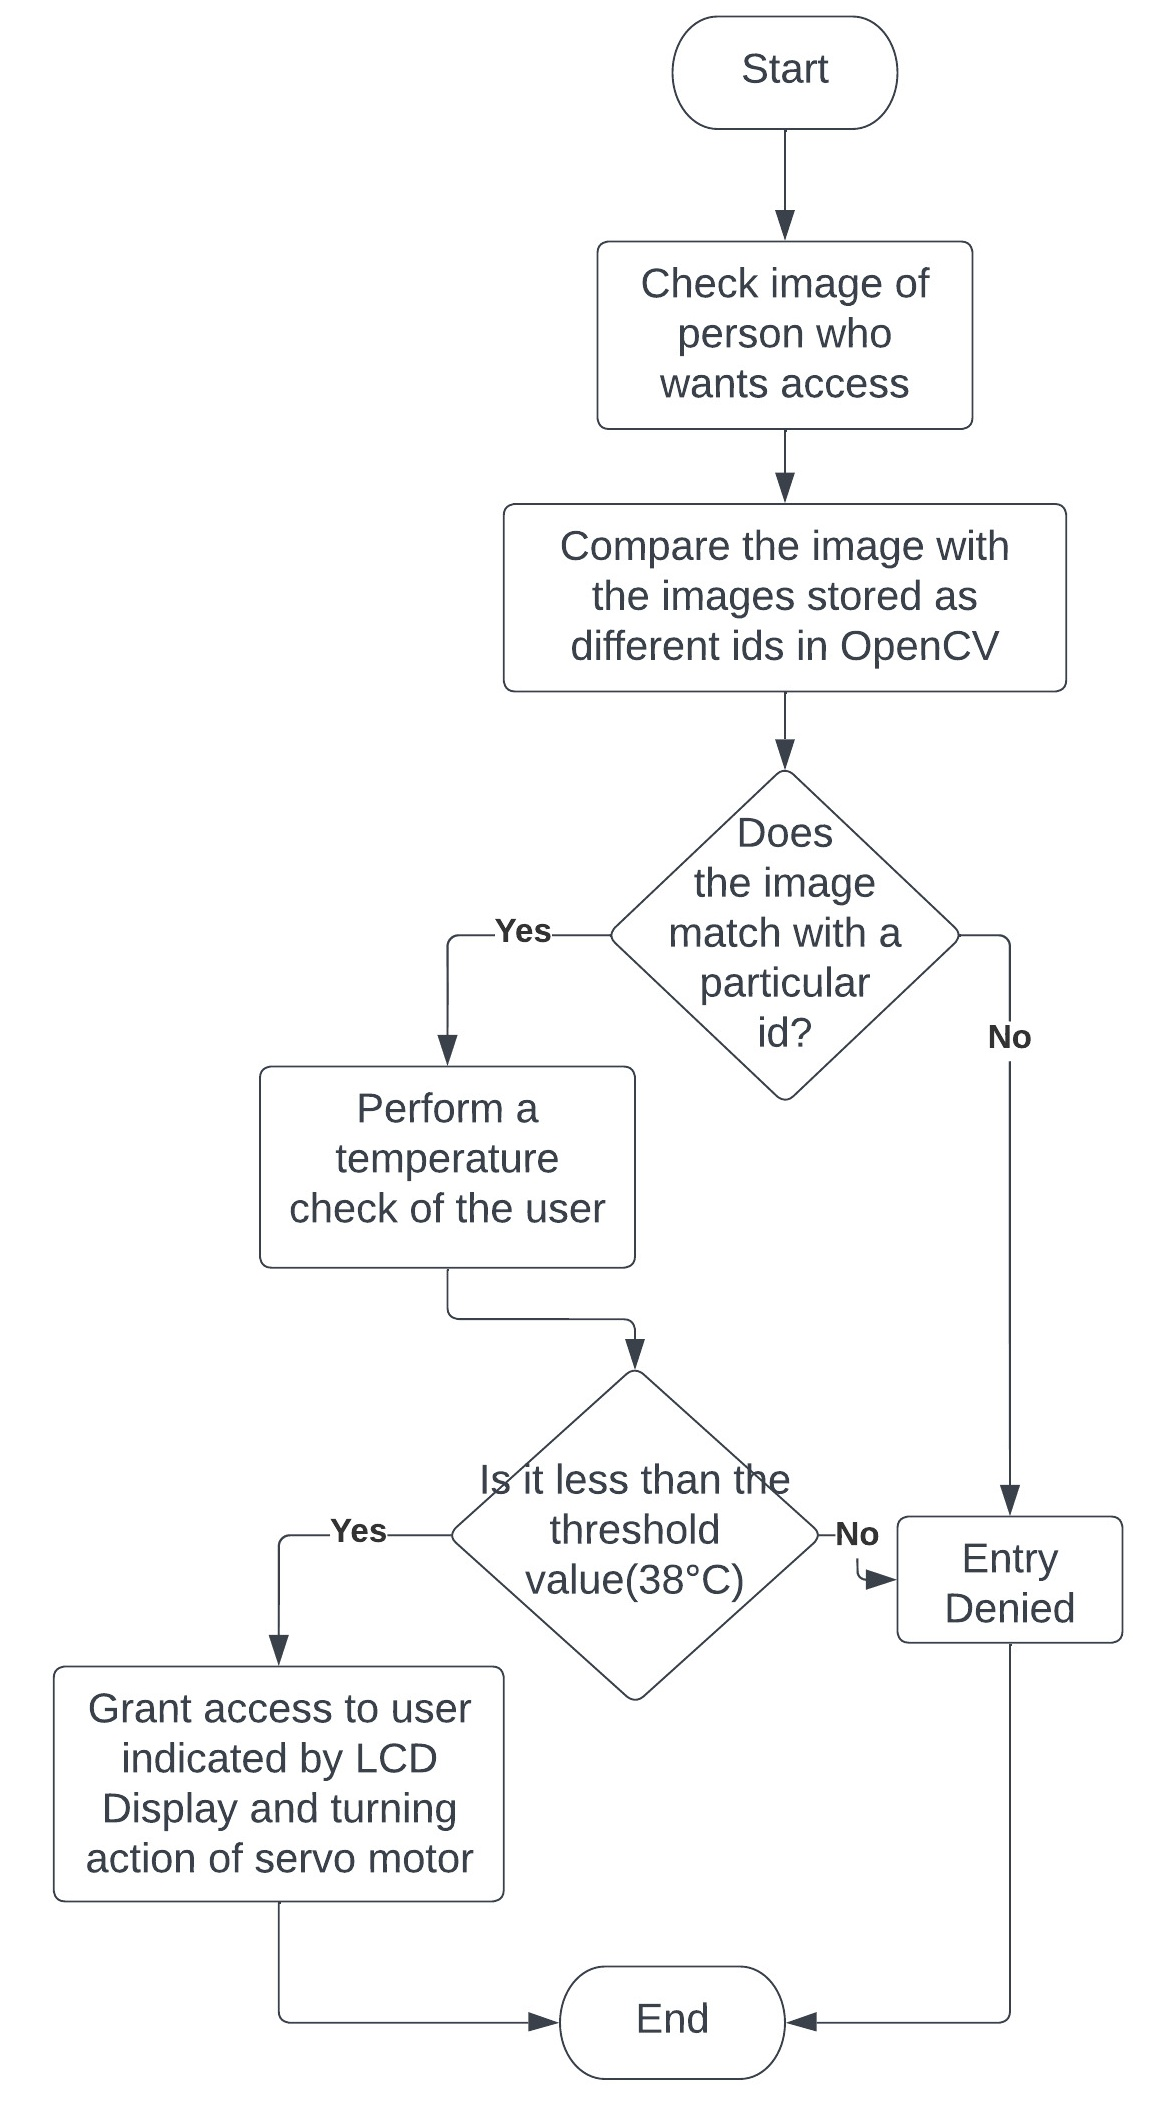
\includegraphics[width=9cm, height=16cm]{flow chart (1).jpg}
		\caption{\label{fig:caption}Flow Chart}
	\end{figure}
	\subsection{Simulation}
	After designing the circuit and employing the necessary
	software applications, the system is ready for simulation. For testing and debugging, the system is first run entirely virtually. The Python script sends the facial recognition data to the Arduino board. Depending on the input received by the temperature sensor, which is adjusted by the user, the Arduino makes the decision of granting or denying access to
	the current user. Two additional software applications may be required depending on whether the system is being run purely as a simulation or is implemented through hardware. During simulation or system testing, the circuit is built of Proteus Simulation Software. All the necessary components are added to the system and the microcontroller is loaded with the code. Along with this, a Virtual Serial Port Emulator is used. It a tool to emulate serial ports for the sake of communication \cite{l}. It allows the pairing of the various ports available on the computer. This allows Python and the microcontroller to interact with each other and send data. During hardware implementation, this is achieved by connected the Arduino to a computer manually and selecting the necessary port to send data over. The circuit consists of the microcontroller, LCD Screen, Servo Motor, LM-35 and a few LEDs \cite{k}. \\\\
	The LCD and LEDs are used as visual indicators for granting or denying access. A servo motor is used to emulate the opening and closing of an automatic door to allow entry. It rotates back to its original position within a few seconds. 
	\begin{figure}
		\centering
		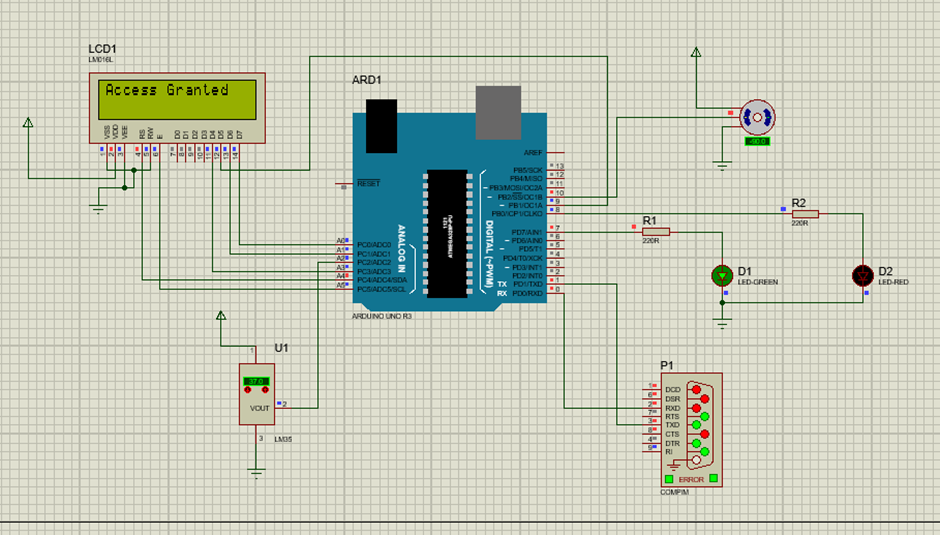
\includegraphics[width=8.5cm, height=5cm]{ProtC1.png}
		\caption{\label{fig:The-caption}Case 1: Access Granted}
	\end{figure}
	\begin{figure}
		\centering
		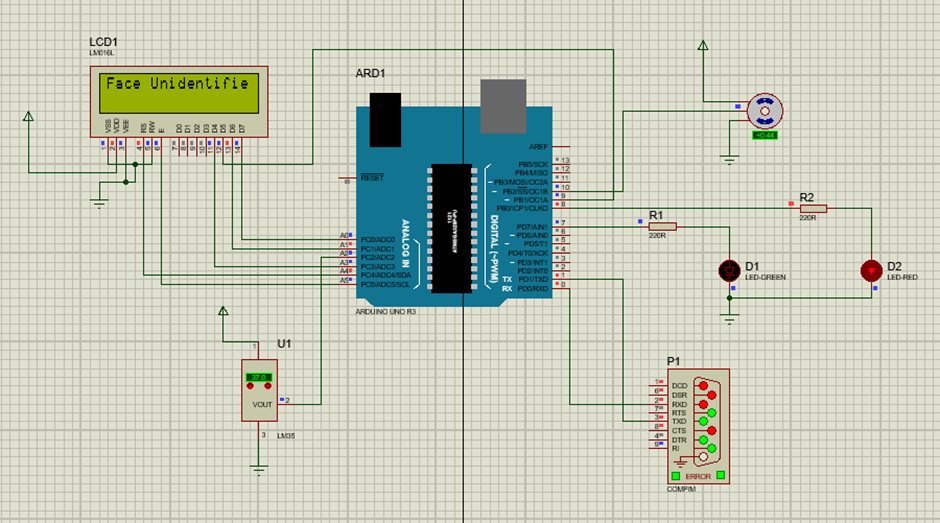
\includegraphics[width=8.5cm, height=5cm]{ProtC2.png}
		\caption{\label{fig:The-caption}Case 2: Access Denied since face is unidentified}
	\end{figure}
	\begin{figure}
		\centering
		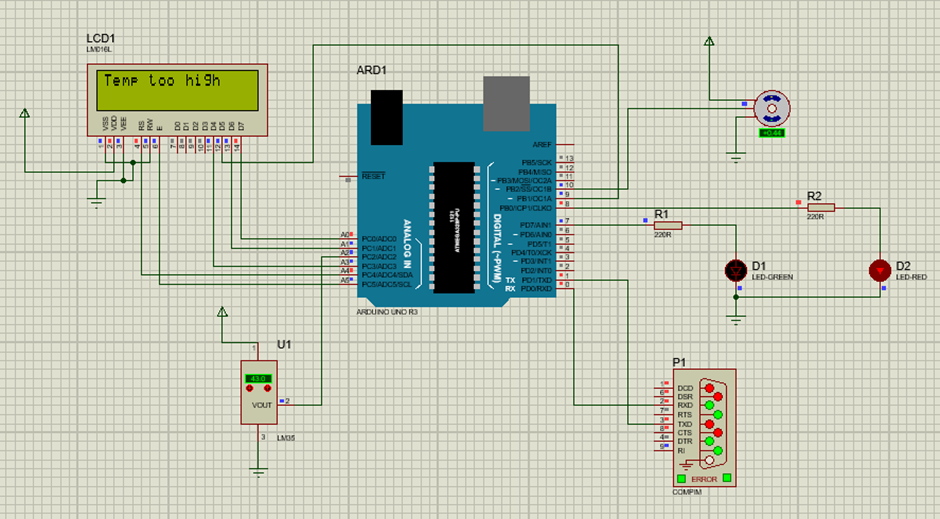
\includegraphics[width=8.5cm, height=5cm]{ProtC3.png}
		\caption{\label{fig:The-caption}Case 3: Access Denied since temperature is too high}
	\end{figure}
	\subsection{Methodology}
	\subsubsection{Facial Recognition System}
	The facial recognition system was made using OpenCV library installed in python wherein the following steps take place \cite{g}.
	\begin{itemize}
		\item Data is gathered and different datasets are made. Each different dataset is given a separate unique id.
		\item With the gathered dataset the recognizer is trained.
		\item Now that the recognizer is trained if the if there is
		an input of a face to the system then the system
		will compare it to the dataset.
		\item If there is a match with any id that has been in the dataset and trained to the recognizer then the face
		will be recognized.\\
	\end{itemize}
	\subsubsection{Temperature Sensing System}
	The temperature sensing
	stem with the help of LM-35 temperature sensor functions
	in the following steps \cite{i}.
	\begin{itemize}
		\item The LM-35 temperature sensor senses the
		temperature of the user.
		\item The analog temperature voltage is converted to a
		digital reading and is sent to the Arduino uno.
		\item The Arduino compares the temperature to the set
		threshold temperature (100 F or 38 C).
		\item If the temperature of the user is less than the
		threshold temperature only then will it be ok to
		grant access.\\
	\end{itemize}
	\subsubsection{Servo Motor}
	The Servo Motor is basically an ordinary motor which simulates an accurate and controlled circular rotation in our system \cite{j}. It is used as mentioned below:
	\begin{itemize}
		\item When we have both our conditions fulfilled, i.e, a match in the facial scan and the body temperature below a certain value, only then will the servo motor be activated and directed to rotate by precisely 90 degrees.
		\item This rotation is used to simulate the unlocking of the door, hence finally granting access to the user.\\\\
	\end{itemize}
	
	
	\section{Results}
	Since we used OpenCV, which requires a dataset of images as training models \cite{f}, we added 100 images of 3 people to our directory. These were analyzed by the algorithm as a set of coordinates and the images were compared with the faces on the webcam. For test purposes, 2 of the faces were detected since they matched with the data in the directory and one was detected as unidentified, thus posing as a security threat.\\
	The values of accuracy are an approximation after running various tests. The loss in accuracy comes primarily from the face recognition system. Its accuracy can be improved by using a camera with better resolution, deploying the system in a well-lit place, and providing a greater set of data to train the model to improve detection.\\
	\begin{figure}
		\centering
		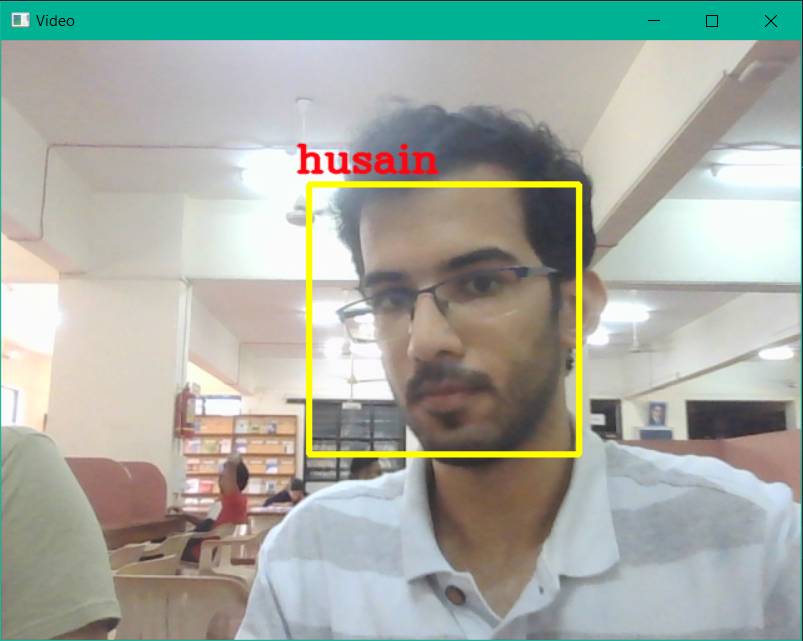
\includegraphics[width=8.5cm, height=7cm]{Husain.png}
		\caption{\label{fig:The-caption}Case 1: Identified Person 1}
	\end{figure}
	\begin{figure}
		\centering
		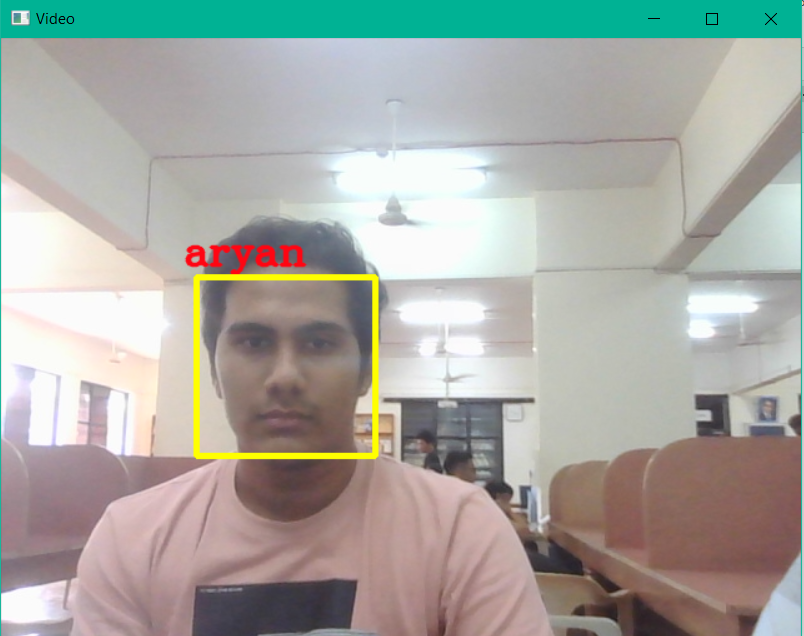
\includegraphics[width=8.5cm, height=7cm]{Aryan.png}
		\caption{\label{fig:The-caption}Case 2: Identified Person 2}
	\end{figure}
	\begin{figure}
		\centering
		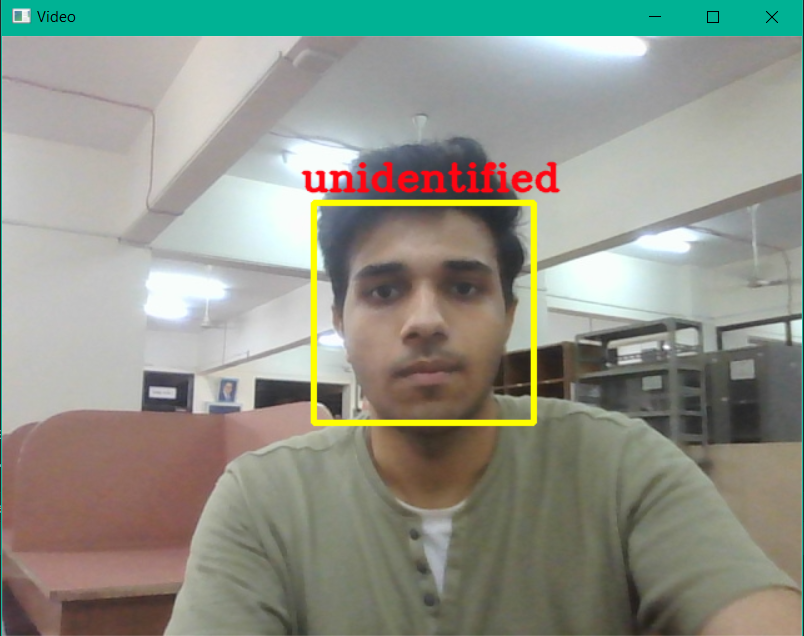
\includegraphics[width=8cm, height=7cm]{Un.png}
		\caption{\label{fig:The-caption}Case 3: Unidentified Person}
	\end{figure}
	\begin{center}
		\caption{Accuracy Table}
		\begin{tabular}{ | m{6em} | m{3cm}| m{2cm} | } 
			\hline
			Test& Result & Accuracy \\ 
			\hline
			Recognized Face
			+ Body
			Temperature
			below 38 C & Access Granted -
			Face identified
			and temperature
			acceptable & 85\% \\ 
			\hline
			Unrecognized
			Face + Body
			Temperature
			below 38 C & Access Denied -
			Face unidentified & 90\% \\ 
			\hline
			Recognized Face
			+ Body
			Temperature
			above 38 C & Access Denied -
			Temperature too
			high & 99\% \\
			\hline
			Unrecognized
			Face + Body
			Temperature
			above 38 C & Access Denied -
			Face unidentified
			and temperature
			too high & 99\% \\
			\hline
		\end{tabular}
		\label{tab:caption}
	\end{center}
	
	\hfill
	\section{Conclusion and Future Scope}
	We have thus successfully simulated a Facial Recognition
	based Security System integrated with an LM-35 Temperature
	Sensor. The primary objective of this project was to provide a security system that eliminated the use of passwords (which may be forgotten and are relatively unsafe and can also be compromised) and fingerprints that can act as a means to spread diseases which is highly unsuitable given the current COVID-19 pandemic situation. The facial recognition system proposed is much more accurate as compared to a fingerprint-based system and since it is combined with a temperature sensor it
	provides an additional check for body temperature which is now a mandatory security parameter in malls and offices worldwide. It also provides for a cost-effective and user-friendly design.\\
	We have used several platforms for our project that perform their specific tasks. Primarily we used a python-based image processing system called OpenCV that uses a webcam to detect the face of a person and identify whether or not the face matches with a set of images provided and stored in its database.\\ Next, we took the help of Arduino to implement our conditional checks of the facial and temperature criteria and display the result accordingly.
	After this, we used a simulation software called Proteus which had our entire circuit board and was meant for displaying our final output using a digital display.\\
	The future scope for this project would be to implement the system using physical components and to integrate it with voice recognition-based software to increase the level of security as well as the complexity to reduce external attacks.
	
	% use section* for acknowledgement
	%\section*{Acknowledgment}
	% optional entry into table of contents (if used)
	%\addcontentsline{toc}{section}{Acknowledgment}
	%We take this opportunity to express our sincere
	%thanks to our guide Prof Anand Mane,
	%Professor of Electronics and Telecommunication
	%Engineering, S.P.I.T., Mumbai, for providing the
	%technical guidelines and the suggestions regarding line the
	%of this work. We would like to express our gratitude
	%towards his constant encouragement, support and
	%guidance throughout the development of the project.
	
	\begin{thebibliography}{1}
		
		\bibitem{a}
		Saghaei, Hamed. (2012). Digital thermometer using LM35 and AVR Microcontroller. 10.13140/RG.2.2.16626.71368. 
		\bibitem{b}
		Raju, Srujan \& Sinha, Professor G. (2020). Automatic Temperature Control System Using Arduino. Advances in Intelligent Systems and Computing. 1090. 219-226. 10.1007/978-981-15-1480-7\_18. 
		\bibitem{c}
		A Arefín, Utsho \& Roy, Vaskar \& Sagar, Md. (2013). Digital Thermometer using ATmega8 Microcontroller. 10.13140/2.1.3551.7763.
		\bibitem{d} 
		Face Detection in Real Time Based on HOG. N. J. Wang,S.
		C. Chang and P. J. Chou. Taipei, Taiwan: IEEE,
		DOI:10.1109/ISPACS.2012.6473506, 2012. International
		Symposium on Intelligent Signal Processing and
		Communications Systems. pp. 333-337. ISBN: 978-1-4673-
		5081-5.
		\bibitem{e} 
		Face Detection and Tracking using OpenCV.
		S.V.Viraktamath, Mukund Katti, Aditya Khatawkar, Pavan
		Kulkarni. 3, s.l.: SIJ, July-August 2013, The Standard
		International Journals (The SIJ) , Vol. 1, pp. 45-50. ISSN: 2321
		– 2403
		\bibitem{f}
		Tejashree Dhawle, Urvashi Ukey \& Rakshandha Choudante. Face Detection and Recognition using OpenCV and Python. International Research Journal of Engineering and Technology (IRJET), Volume: 07 Issue: 10 | Oct 2020 
		\bibitem{g}
		Mahamkali, Naveenkumar \& Ayyasamy, Vadivel. (2015). OpenCV for Computer Vision Applications. 
		\bibitem{h} 
		Louis, Leo. (2018). Working Principle of Arduino and Using it as a Tool for Study and Research. International Journal of Control, Automation, Communication and Systems. 1. 10.5121/ijcacs.2016.1203. 
		\bibitem{i} 
		Admin, “Temperature measurement using LM35 and AVR microcontroller,” MaxPhi, 16-Sep-2017. [Online]. Available: https://www.maxphi.com/temperature-measurement-using-lm35-and-avr-microcontroller. [Accessed: 02-Apr-2022]. 
		\bibitem{j}
		Admin, “Temperature measurement using LM35 and AVR microcontroller,” MaxPhi, 16-Sep-2017. [Online]. Available: https://www.maxphi.com/temperature-measurement-using-lm35-and-avr-microcontroller. [Accessed: 02-Apr-2022]. 
		“Servo Motor SG-90,” Components101. [Online]. Available: https://components101.com/motors/servo-motor-basics-pinout-datasheet. [Accessed: 02-Apr-2022].
		\bibitem{k}
		“16x2 LCD display module,” Circuit Digest, 17-Jul-2018. [Online]. Available: https://circuitdigest.com/article/16x2-lcd-display-module-pinout-datasheet. [Accessed: 02-Apr-2022]. 
		\bibitem{l}
		“DB9 changer datasheet PDF,” DB9 Datasheet | ETC - Datasheetspdf.com. [Online]. Available: https://datasheetspdf.com/datasheet/DB9.html. [Accessed: 02-Apr-2022]. 
		
	\end{thebibliography}
\end{document}



